\documentclass[a4paper,nobib]{tufte-book}

\hypersetup{colorlinks}% uncomment this line if you prefer colored hyperlinks (e.g., for onscreen viewing)

%%
% If they're installed, use Bergamo and Chantilly from www.fontsite.com.
% They're clones of Bembo and Gill Sans, respectively.
%\IfFileExists{bergamo.sty}{\usepackage[osf]{bergamo}}{}% Bembo
%\IfFileExists{chantill.sty}{\usepackage{chantill}}{}% Gill Sans

%\usepackage[protrusion=true,expansion,babel=true]{microtype}

%%
% Just some sample text
\usepackage{lipsum}

%%
% For nicely typeset tabular material
\usepackage{booktabs}
\usepackage{multirow}
\usepackage{adjustbox}
\usepackage{array}

\newcolumntype{L}[1]{>{\noindent\RaggedRight\arraybackslash\hspace{0pt}}p{#1}}
\newcolumntype{R}[1]{>{\noindent\RaggedLeft\arraybackslash\hspace{0pt}}p{#1}}
\newcolumntype{C}[1]{>{\noindent\Centering\arraybackslash\hspace{0pt}}p{#1}}

%%
% For graphics / images
\usepackage{graphicx}
\setkeys{Gin}{width=\linewidth,totalheight=\textheight,keepaspectratio}
\graphicspath{{media/}}

% What
\setcounter{secnumdepth}{3}
\setcounter{tocdepth}{3}

% Bibliography
\usepackage[
style=ieee,
citestyle=numeric-comp,
autocite=inline,
autopunct=true,
backend=biber,
maxbibnames=99,
maxcitenames=2,
mincitenames=1,
]{biblatex}
\addbibresource{bibliography.bib}


%%
% Maths
\usepackage{amsmath}

% Prints a trailing space in a smart way.
\usepackage{xspace}

% Inserts a blank page
\newcommand{\blankpage}{\newpage\hbox{}\thispagestyle{empty}\newpage}

% Referencing
\usepackage[unicode]{hyperref}
\usepackage[nameinlink]{cleveref}

\hypersetup{%
	bookmarksnumbered = true, % Show section numbering in the PDF table of contents. Allows easier browsing of the document
	colorlinks = true, % uncomment this line if you prefer colored hyperlinks (e.g., for onscreen viewing)
%	pdfborder = {0 0 0},
	bookmarksdepth = subsection,
%	citecolor = DarkGreen,
%	linkcolor = DarkBlue,
%	urlcolor = DarkGreen,
}

%\AtBeginDocument{%
%	\hypersetup{
%		pdfauthor={\plainauthor}
%		pdftitle={\plaintitle},
%	}%
%}

\usepackage[binary-units=true]{siunitx}

% Modifications to the default tufte template to make it more applicable to a thesis
% Credit goes to Tiffany Tseng, lalider, see https://github.com/lalider/tufte-latex-thesis

\usepackage[parfill]{parskip}

% remove paragraph indentation
\makeatletter
% Paragraph indentation and separation for normal text
\renewcommand{\@tufte@reset@par}{%
	\setlength{\RaggedRightParindent}{0.0pc}%
	\setlength{\JustifyingParindent}{0.0pc}%
	\setlength{\parindent}{0pc}%
	\setlength{\parskip}{\baselineskip}%
}
\@tufte@reset@par

% Paragraph indentation and separation for marginal text
\renewcommand{\@tufte@margin@par}{%
	\setlength{\RaggedRightParindent}{0.0pc}%
	\setlength{\JustifyingParindent}{0.0pc}%
	\setlength{\parindent}{0.0pc}%
	\setlength{\parskip}{10pt}%
}
\makeatother

\titleformat{\section}%
[hang]% shape
{\normalfont\Large}% format applied to label+text
{\thesection}% label
{1em}% horizontal separation between label and title body
{}% before the title body
[]% after the title body

%\titlespacing*{\section}{0pt}{3.5ex plus 1ex minus .2ex}{2.3ex plus .2ex}
%\titlespacing*{\subsection}{0pt}{3.25ex plus 1ex minus .2ex}{1.5ex plus.2ex}
\titlespacing*{\section}{0pt}{30pt}{20pt}
\titlespacing*{\subsection}{0pt}{20pt}{5pt}


% Disable adding empty pages without a purpose (not intended for printing in a book format...)
\makeatletter
\def\cleardoublepage{
	\clearpage%
}
\makeatother

% Acronyms
\usepackage{acro}
\acsetup{
	use-id-as-short,
	make-links=false,
	case-sensitive=false,
	patch/floats=false,
	patch/caption=false,
	patch/tabularx=false
}
\DeclareAcronym{FDIR}{short=FDIR,long={Fault Detection, Isolation and Recovery}}
\DeclareAcronym{ADCS}{short = ADCS, long = {Attitude Determination and Control Subsystem}}
\DeclareAcronym{COMMS}{short = COMMS, long = {Communications}}
\DeclareAcronym{EPS}{short = EPS, long = {Electrical Power Subsystem}}
\DeclareAcronym{OBC}{short = OBC, long = {On-Board Computer}}
\DeclareAcronym{OBDH}{short = OBDH, long = {On-Board Data Handling}}
\DeclareAcronym{OBSW}{short = OBSW, long = {On-Board Software}}
\DeclareAcronym{OPS}{short = OPS, long = {Operations}}
\DeclareAcronym{SYE}{short = SYE, long = {Systems Engineering}}
\DeclareAcronym{SU}{short = SU, long = {Science Unit}}
\DeclareAcronym{EMC}{short = EMC, long = {Electromagnetic Compatibility}}
\DeclareAcronym{CDR}{short = CDR, long = {Critical Design Review}}
\DeclareAcronym{GS}{short = GS, long = {Ground Station}}
\DeclareAcronym{TC}{short = TC, long = Telecommands}
\DeclareAcronym{TM}{short = TM, long = Telemetry}
\DeclareAcronym{RF}{short = RF, long = RadioFrequency}
\DeclareAcronym{CCSDS}{short = CCSDS, long = {The Consultative Committee for Space Data Systems}}
\DeclareAcronym{ISM}{short = ISM, long = {Industrial, Scientific, Medical}}
\DeclareAcronym{COTS}{short = COTS, long = {Commercial Off-The-Shelf}}
\DeclareAcronym{PCDU}{short = PCDU, long = {Power Conditioning \& Distribution Unit}}
\DeclareAcronym{MPPT}{short = MPPT, long = {Maximum Power Point Tracking}}
\DeclareAcronym{ECSS}{short = ECSS, long = {European Cooperation for Space Standardization}}
\DeclareAcronym{PUS}{short = PUS, long = {Packet Utilisation Standard}}
\DeclareAcronym{UHF}{short = UHF, long = {Ultra-High Frequency}}
\DeclareAcronym{LEO}{short = LEO, long = {Low Earth Orbit}}
\DeclareAcronym{PDMS}{short = PDMS, long = {Polydimethylsiloxane}}
\DeclareAcronym{PA}{short = PA, long = {Product Assurance}}
\DeclareAcronym{PCB}{short = PCB, long = {Printed Circuit Board}}
\DeclareAcronym{GMAT}{short = GMAT, long = {General Mission Analysis Tool}}
\DeclareAcronym{MRAM}{short = MRAM, long = {Magnetoresistive Random-Access Memory}}
\DeclareAcronym{CAN}{short = CAN, long = {Controller Area Network}}
\DeclareAcronym{MCU}{short = MCU, long = {microcontroller}, extra={MicroController Unit}}
\DeclareAcronym{RTOS}{short = RTOS, long = {Real-Time Operating System}}
\DeclareAcronym{SAVOIR}{short = SAVOIR, long = {Space AVionics Open Interface aRchitecture}}
\DeclareAcronym{YAMCS}{short = YAMCS, long = {Yet Another Mission Control System}}
\DeclareAcronym{COBS}{short = COBS, long = {Consistent Overhead Byte Stuffing}}
\DeclareAcronym{SRAM}{short = SRAM, long = {Static Random Access Memory}}
\DeclareAcronym{I2C}{short = {I\textsuperscript{2}C}, long = {Inter-Integrated Circuit}}
\DeclareAcronym{ETL}{short = ETL, long = {Embedded Template Library}}
\DeclareAcronym{HAL}{short = HAL, long = {Hardware Abstraction Library}}
\DeclareAcronym{IDE}{short = IDE, long = {Integrated Development Environment}}
\DeclareAcronym{USB}{short = USB, long = {Universal Serial Bus}}
\DeclareAcronym{UART}{short = UART, long = {Universal Asynchronous Serial Bus}}
\DeclareAcronym{FMEA}{short = FMEA, long = {Failure Mode and Effects Analysis}}
\DeclareAcronym{FMECA}{short = FMECA, long = {Failure Mode, Effects and Criticality Analysis}}
\DeclareAcronym{HSIA}{short = HSIA, long = {Hardware/Software Interaction Analysis}}
\DeclareAcronym{XTCE}{short = XTCE, long = {XML Telemetric and Command Exchange}}
\DeclareAcronym{RAMS}{short = RAMS, long = {Reliability, Availability, Maintainability and Safety}}
\DeclareAcronym{MAIV}{short = MAIV, long = {Maintenance, Assembly, Integration and Verification}}
\DeclareAcronym{IC}{short = IC, long = {Integrated Circuit}}
\NewDocumentCommand\draft{m}{%
	\textcolor[HTML]{bf616a}{#1}%
}

\makeatletter
\newcommand\footurl@[1]{\footnote{\url@{#1}}}
\DeclareRobustCommand{\footurl}{\hyper@normalise\footurl@}

\newcommand\foothref@[2]{\href@{#1}{#2}\footnote{\url@{#1}}}
\def\Hy@foothref#{%
	\hyper@normalise\foothref@
}
\DeclareRobustCommand*{\foothref}[1][]{%
	\begingroup
	\setkeys{href}{#1}%
	\@ifnextchar\bgroup\Hy@foothref{\hyper@normalise\foothref@}%
}
\makeatother

% Transitions
\AtBeginDocument{
\colorlet{invalid}{MaterialAmber900}
\colorlet{unexpected}{MaterialRed900}
}

\def\unchecked{\textcolor{MaterialGrey800}{\texttt{Unchecked}}}
\def\ok{\texttt{OK}}
\def\unexpected{\textcolor{unexpected}{\texttt{Unexpected\_Value}}}
\def\hilim{\textcolor{unexpected}{\texttt{Above\_High\_Limit}}}
\def\lolim{\textcolor{unexpected}{\texttt{Below\_Low\_Limit}}}
\def\invalid{\textcolor{invalid}{\texttt{Invalid}}}
\def\ar{ \( \rightarrow \) }

\makeatletter

\makeatother

\NewAcroTemplate[list]{glossary}{%
	\begin{description}
		\acronymsmapF{%
			\item[\sffamily\textbf{\acrowrite{short}}] \acrowrite{long}%
			\acroifanyT {foreign,extra} {~(}%
			\acrowrite {foreign}%
			\acroifallT {foreign,extra} {,~}%
			\acrowrite {extra}%
			\acroifanyT {foreign,extra} {)}%
			\acropagefill%
			\acropages%
				{ \acrotranslate {page} \nobreakspace }%
				{ \acrotranslate {pages} \nobreakspace }%
		}%
		{ \item \AcroRerun{list} }%
		\end {description}
	}

% Various utilities
\usepackage{tabularx}
\usepackage[singlelinecheck=false]{caption}
\usepackage{subcaption}
\usepackage{comment}

% Generates the index
\usepackage{makeidx}
\makeindex

\usepackage{tikz}
\usepackage{pgfplots}
\pgfplotsset{compat = 1.3}
\usetikzlibrary{pie}
\usepackage{physics}
\let\Re=\relax
\let\Im=\relax

% Colours
\definecolor{off}{HTML}{e53935}
\definecolor{on}{HTML}{43a047}
\usepackage{xcolor-solarized}
\usepackage{xcolor-material}
\usepackage{colortbl}

%\usepackage{todonotes}
\usepackage{enumitem}
\usepackage[absolute,overlay]{textpos}

% Code
\usepackage{minted}
\usepackage{xpatch,letltxmacro}
\LetLtxMacro{\cminted}{\minted}
\let\endcminted\endminted
\xpretocmd{\cminted}{\RecustomVerbatimEnvironment{Verbatim}{BVerbatim}{}}{}{}
\definecolor{mintedbg}{rgb}{0.95,0.95,0.93}
\setminted{
	bgcolor=mintedbg,
	tabsize=2
}
\setminted[text]{baselinestretch=0.8}

% Git magic
\makeatletter
\write18{git log --pretty='format:\@percentchar Creset\@percentchar s' --no-merges -1 > \jobname.git1.tmp}
\write18{git rev-parse --short HEAD > \jobname.git2.tmp}
\def\gitcommit{\input{\jobname.git2.tmp}\unskip}
\def\gitcommitmessage{\input{\jobname.git1.tmp}\unskip}
\makeatother

% Smart citations

\makeatletter

%\def\blx@imc@mkbibquote{\blx@enquote}

\newbibmacro*{cite:title}{%
  \printtext[bibhyperref]{%
    \printfield[citetitle]{labeltitle}}%
  \finentry}

\newbibmacro*{cite:shorthand}{%
	\printtext[bibhyperref]{\printfield{shorthand}}}

\newbibmacro*{cite:full}{%
	\iffieldundef{shorthand}
	{\printnames{labelname}%
		\setunit*{\printdelim{nametitledelim}}%
		\usebibmacro{cite:title}}%
	{\usebibmacro{cite:shorthand}}}

\newbibmacro*{cite:marginnote}{%
	\marginnote{%
		% \mkbibbrackets should be used here probably
		[%
			\printfield{labelprefix}%
			\printfield{labelnumber}%
		]
		\usebibmacro{cite:full}%
	}%
}

\DeclareCiteCommand{\dualcite}[\mkbibbrackets]
  {\usebibmacro{cite:init}%
   \usebibmacro{prenote}}
  {\usebibmacro{citeindex}%
   \usebibmacro{cite:marginnote}%
   \usebibmacro{cite:comp}}%
  {}
  {\usebibmacro{cite:dump}%
   \usebibmacro{postnote}}

\def\tuftecite{
	\iffootnote{footnote}{text}
}

% Patching commands that enter information in margins, so that we can detect which
% citation should be used
\newtoggle{inmargin}
\pretocmd{\marginpar}{\toggletrue{inmargin}}{}{}
\apptocmd{\@xympar}{\togglefalse{inmargin}}{}{}
\pretocmd{\@tufte@float}{\toggletrue{inmargin}}{}{}
\pretocmd{\end@tufte@float}{\togglefalse{inmargin}}{}{}
\pretocmd{\@tufte@margin@float}{\toggletrue{inmargin}}{}{}
\pretocmd{\end@tufte@margin@float}{\togglefalse{inmargin}}{}{}

\def\autocite{%
	\iftoggle{inmargin}\parencite\dualcite%
}

% Tufte disables subparagraphs. This brings them back.
\renewcommand\subparagraph{\@startsection{subparagraph}{5}{\parindent}%
	{3.25ex \@plus1ex \@minus .2ex}%
	{-1em}%
	{\hspace{1em}\normalfont\normalsize\itshape}}

% \acuse command that also adds the current page
%\NewAcroTemplate{fdirthesisempty}{}
%\NewAcroCommand\acusepage{m}{}
\let\acusepage\acuse

\makeatother

%%
% Book metadata
\title{Design of Fault Detection, Isolation and Recovery in the AcubeSAT nanosatellite\thanks{AcubeSAT}}
\author[kongr45gpen]{kongr45gpen}
\publisher{Draft SpaceDot}

\begin{document}

% Front matter
%\frontmatter

% r.1 blank page
%\blankpage

% r.3 full title page
\maketitle


% v.4 copyright page
\newpage
\begin{fullwidth}
~\vfill
\thispagestyle{empty}
\setlength{\parindent}{0pt}
\setlength{\parskip}{\baselineskip}
Copyright \copyright\ \the\year\ \thanklessauthor

\par\smallcaps{Published by \thanklesspublisher}

\par\smallcaps{tufte-latex.github.io/tufte-latex/}

\par Licensed under the Apache License, Version 2.0 (the ``License''); you may not
use this file except in compliance with the License. You may obtain a copy
of the License at \url{http://www.apache.org/licenses/LICENSE-2.0}. Unless
required by applicable law or agreed to in writing, software distributed
under the License is distributed on an \smallcaps{``AS IS'' BASIS, WITHOUT
WARRANTIES OR CONDITIONS OF ANY KIND}, either express or implied. See the
License for the specific language governing permissions and limitations
under the License.\index{license}

\par The AcubeSAT project is carried out with the support of the Education Office of the \href{https://www.esa.int/}{European Space Agency}, under the educational \href{https://www.esa.int/Education/CubeSats_-_Fly_Your_Satellite/}{Fly Your Satellite! programme}.

\par The views expressed herein by the authors can in no way be taken to reflect the official opinion, or endorsement, of the European Space Agency.

\par\textit{First printing, 2021}
\end{fullwidth}

% r.5 contents
\tableofcontents

\listoffigures

\listoftables

%\chapter*{List of Acronyms}
%\acuseall%
\printacronyms[pages={display=all,seq/use=false}]

% r.9 introduction
\cleardoublepage

\chapter*{Abstract}

%This sample book discusses the design of Edward Tufte's
%books\cite{Tufte2001,Tufte1990,Tufte1997,Tufte2006}.
\justify
Space is not a welcoming environment; while the aerospace engineering community has managed to reliably operate thousands of satellites in orbit, CubeSats, the most popular class of nanosatellite, only have a 50\% success rate. Low costs, lack of strict technical requirements and scarcity of publicly available documentation often drives up the risks for educational, scientific and commercial CubeSats. This thesis investigates a configurable and modular Fault Detection, Isolation and Recovery (FDIR) architecture that uses the ECSS Packet Utilisation Standard. This FDIR concept, along with the provided open-source software implementation, can be used by CubeSat missions to increase the reliability of their design and chances of mission success, by autonomously responding to on-board errors. The thesis also includes background information regarding CubeSat reliability, and explores the software and hardware used to implement the proposed FDIR design on the AcubeSAT mission, currently under design by students of the Aristotle University of Thessaloniki.



%%
% Start the main matter (normal chapters)
\mainmatter


\chapter{Reliability Engineering in CubeSat Systems}
\label{sec:fdir}


%\newthought{The pages} of a book are usually divided into three major
%sections: the front matter (also called preliminary matter or prelim), the
%main matter (the core text of the book), and the back matter (or end
%matter).

%\newthought{The front matter} of a book refers to all of the material that
%comes before the main text.  The following table from shows a list of
%material that appears in the front matter of
%along with its page number.  Page numbers that appear in parentheses refer
%to folios that do not have a printed page number (but they are still
%counted in the page number sequence).

\section{Kalispera}
space is very important \autocite{durou_hierarchical_2002}
\acf{FDIR}

\chapter{The AcubeSAT mission}

\section{CubeSat}


\section{Subsystems}

The AcubeSAT nanosatellite is technically and programmatically split into \draft{N} different subteams or \textbf{subsystems}, each responsible for a different section of the satellite, and made up out of \draft{M} dedicated members.

In the following sections, a brief introduction on the function and design of each subsystem is presented. For more detailed information, the reader is encouraged to refer to \foothref{https://acubesat.spacedot.gr/subsystems/}{AcubeSAT's website}, or to the publicly available \foothref{https://gitlab.com/acubesat/documentation/cdr-public}{\ac{CDR} documents}.
\subsection{\acf{ADCS}}

\subsection{\acf{COMMS}}

The communications subsystem is responsible for transmitting data between the Earth and the spacecraft in orbit. The transmitted data is split into 3 different categories:
\begin{itemize}
	\item \textbf{\acf{TC}}: Commands from the Earth to the satellite. They can be used to request information, or to perform specific spacecraft actions.
	\item \textbf{\acf{TM}}: Information sent from the satellite towards Earth, typically including vital information such as sensor values, system status, timestamps and events.
	\item \textbf{Science data}: The scientific data generated by the payload. These are the highest-volume data and represent the main scientific output of the mission.
\end{itemize}

It is important to mention that the satellite orbit only allows for a very short visibility duration every day, increasing the needs for on-board autonomy and the importance of a correctly implemented \acs{FDIR} method.

\begin{marginfigure}
	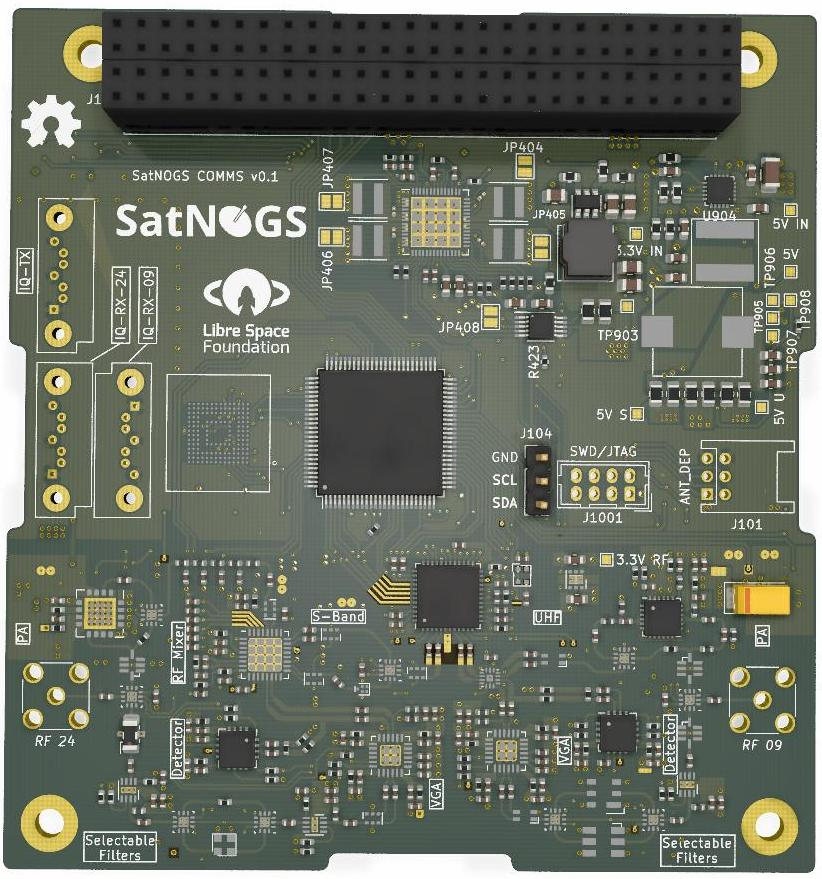
\includegraphics{satnogs-comms}
	\caption{The SatNOGS COMMS board}
\end{marginfigure}

The main component of the \acs{COMMS} subsystems is the \textbf{SatNOGS COMMS board} \autocite{surligas_satnogs-comms_2021}, an open-source \acs{RF} transceiver developed by the \href{https://libre.space/}{LibreSpace Foundation}, based on \acs{CCSDS} telecommunications standards.

Communication will take place using 2 frequency bands on the \acs{ISM} range, namely \SI{436.5}{\mega\hertz} and \SI{2.425}{\giga\hertz}, supported by a deployable turnstile and a directional patch antenna respectively. The use of \acs{ISM} frequencies allows easy radio-amateur access to the satellite.

The communications subsystem is also responsible for the \ac{EMC} analysis and interference mitigation, as well as the design and construction of the satellite \acl{GS}. The \acl{GS} will be part of \textbf{SatNOGS}\autocite{white_overview_2018}, a global network of satellite ground stations based on open technologies and open data.

\subsection{\acf{EPS}}
The \ac{EPS} is the subsystem responsible for the generation, distribution and storage of electrical power of the spacecraft. It is a critical aspect of the spacecraft due to the direct dependence of all subsystems to the high power needs of many CubeSat subsystems, and is theorised to be the most common reason for CubeSat failure.\autocite{langer_reliability_2016}.

AcubeSAT has opted for a \ac{COTS} subsystem approach for the \ac{EPS}:
\begin{itemize}
	\item \textbf{Solar panels} are procured from EnduroSat. Four 3U panels cover the \(X\) and \(Y\) faces of the satellite, and one 1U panel covers the \(-Z\) face.
	\item The \textbf{\ac{PCDU}} is procured from NanoAvionics and offers 10 switched channels with overcurrent protection over 4 voltage rails, as well as 4 \ac{MPPT} converters.
	\item The \textbf{battery pack}, also procured from NanoAvionics, contains 4 18650 Li-Ion cells in a 2S2P\footnote{2 series, 2 parallel} configuration.
\end{itemize}

\subsection{\acf{OBDH}}

\subsection{\acf{OPS}}

\subsection{Structural}

\subsection{\acf{SYE}}

\subsection{\acf{SU}}

\subsection{Thermal}

\subsection{Trajectory}

\section{Tools used}

\chapter{\ac{FDIR} concept in AcubeSAT}

\chapter{Software implementation of \ac{FDIR}}

\chapter{Hardware implementation of \ac{FDIR}}


\backmatter

\printbibliography


\printindex

\end{document}

